\documentclass[
	a4paper,
	12pt,
	brazilian
]{article}

\usepackage[utf8]{inputenc}
\usepackage[T1]{fontenc}

\usepackage{amsmath, amsfonts, amssymb}
\usepackage{siunitx}

\usepackage[
top=2cm,
right=3cm,
bottom=2cm,
left=3cm
]{geometry}

\usepackage{xcolor}
\usepackage{tikz}
\usepackage{import}
\usepackage{float}

\usepackage{graphicx}
\usepackage{hyperref}
\usepackage{cleveref}
\usepackage{bm}
\usepackage{multirow}
\usepackage{cancel}
\usepackage[version=4]{mhchem}

\usepackage{config}

\begin{document}
	\section{Primeira questão}
	Calcular a pressão relativa no ponto indicado da tubulação. Resposta em \SI{}{\pascal} com uma casa decimal.\\\vspace{.5cm}
	
	\textbf{Dados:}
	\begin{itemize}
		\item Massa específica do fluido 1 = $\SI{13.1}{\gram/\centi\meter^{3}}$
		\item Massa específica do fluido 2 = $\SI{8.3}{\gram/\centi\meter^{3}}$
		\item Massa específica da água = $\SI{1000}{\kilogram/\meter^{3}}$
		\item $X=\SI{18.4}{\centi\meter}$
		\item $Y=\SI{8.3}{\centi\meter}$
		\item $Z=\SI{21.9}{\centi\meter}$
		\item $\beta=\SI{67.4}{\SIUnitSymbolDegree}$
	\end{itemize}
	\vspace{-8cm}
	\begin{flushright}
			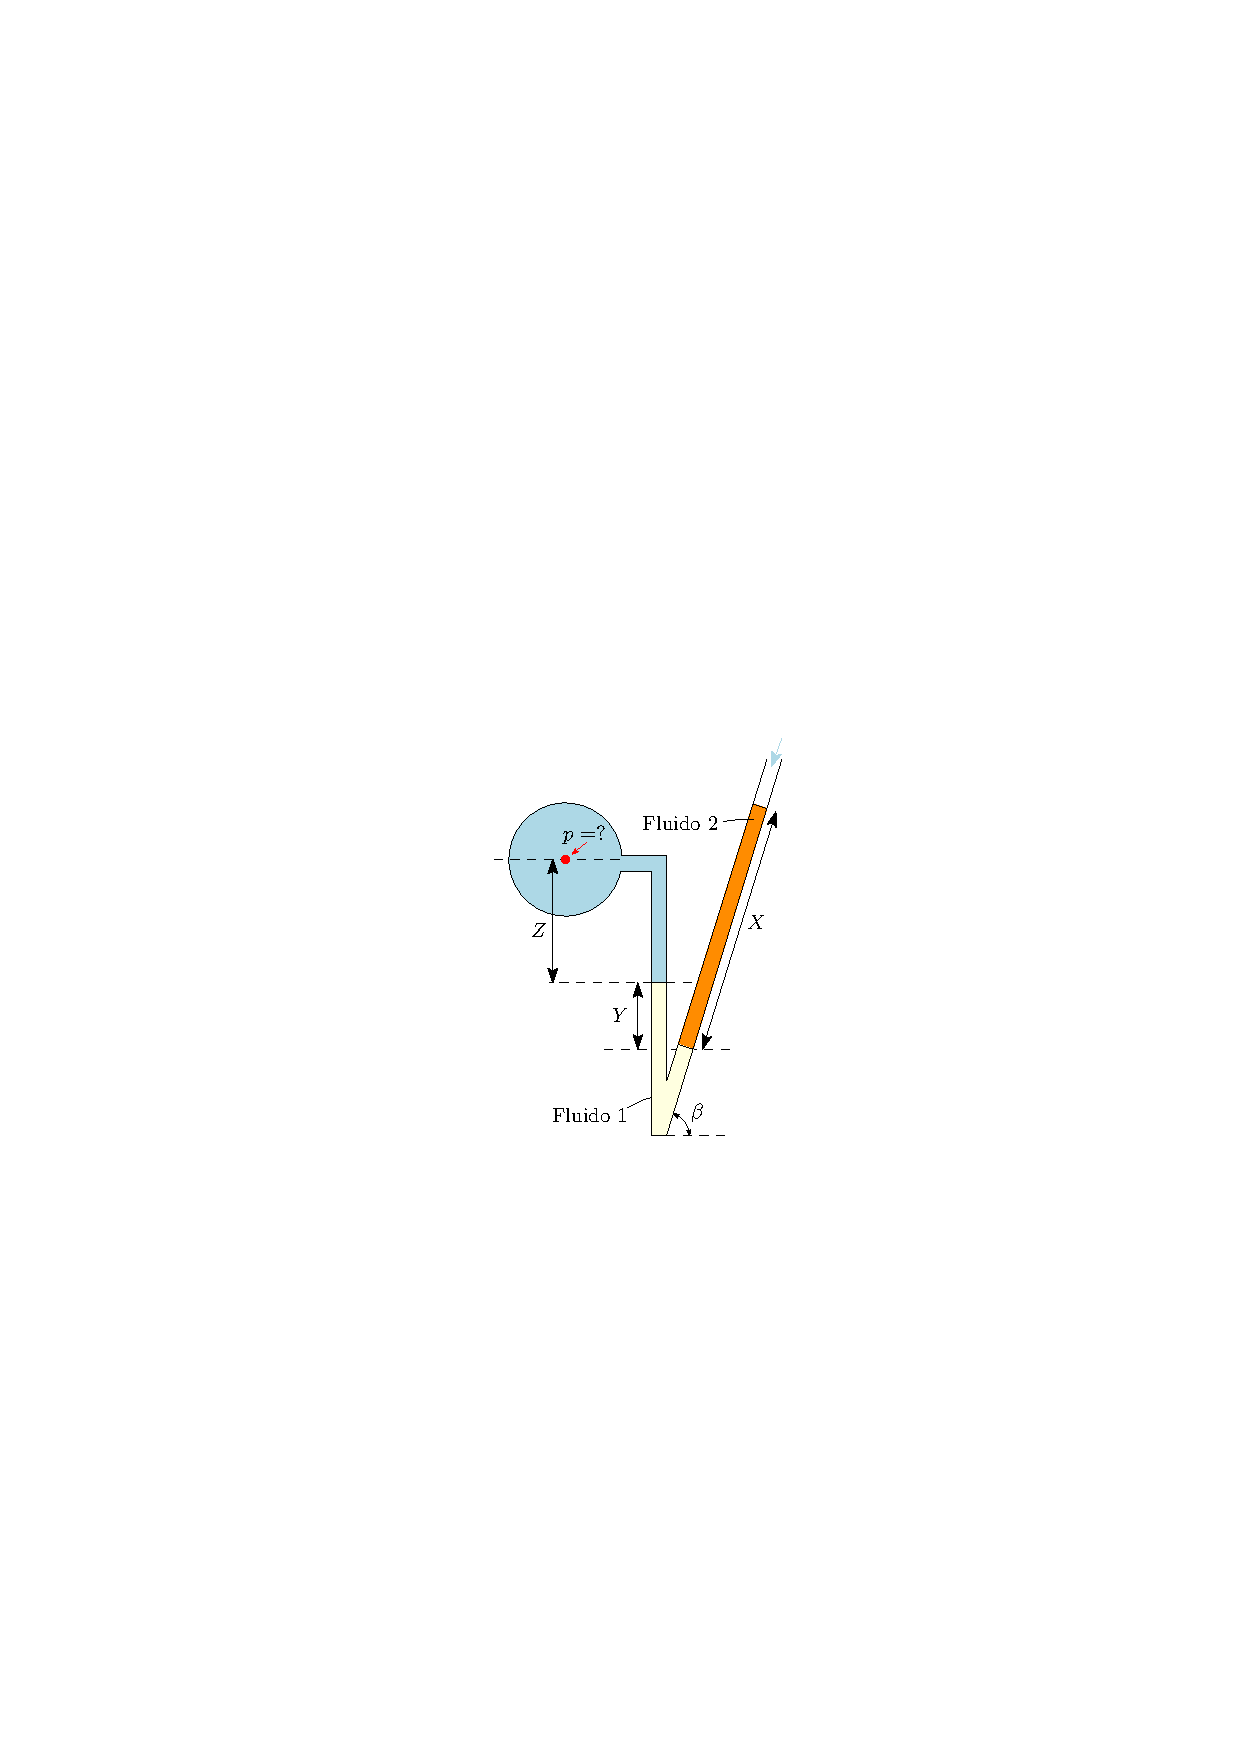
\includegraphics[width=0.4\linewidth]{assets/images/ex1}
	\end{flushright}
	\subsection{Solução}
	\begin{enumerate}
		\item[(1)] Estabelecer um referencial. É comum adotar a interface líquido-líquido mostrada.
		\begin{center}
			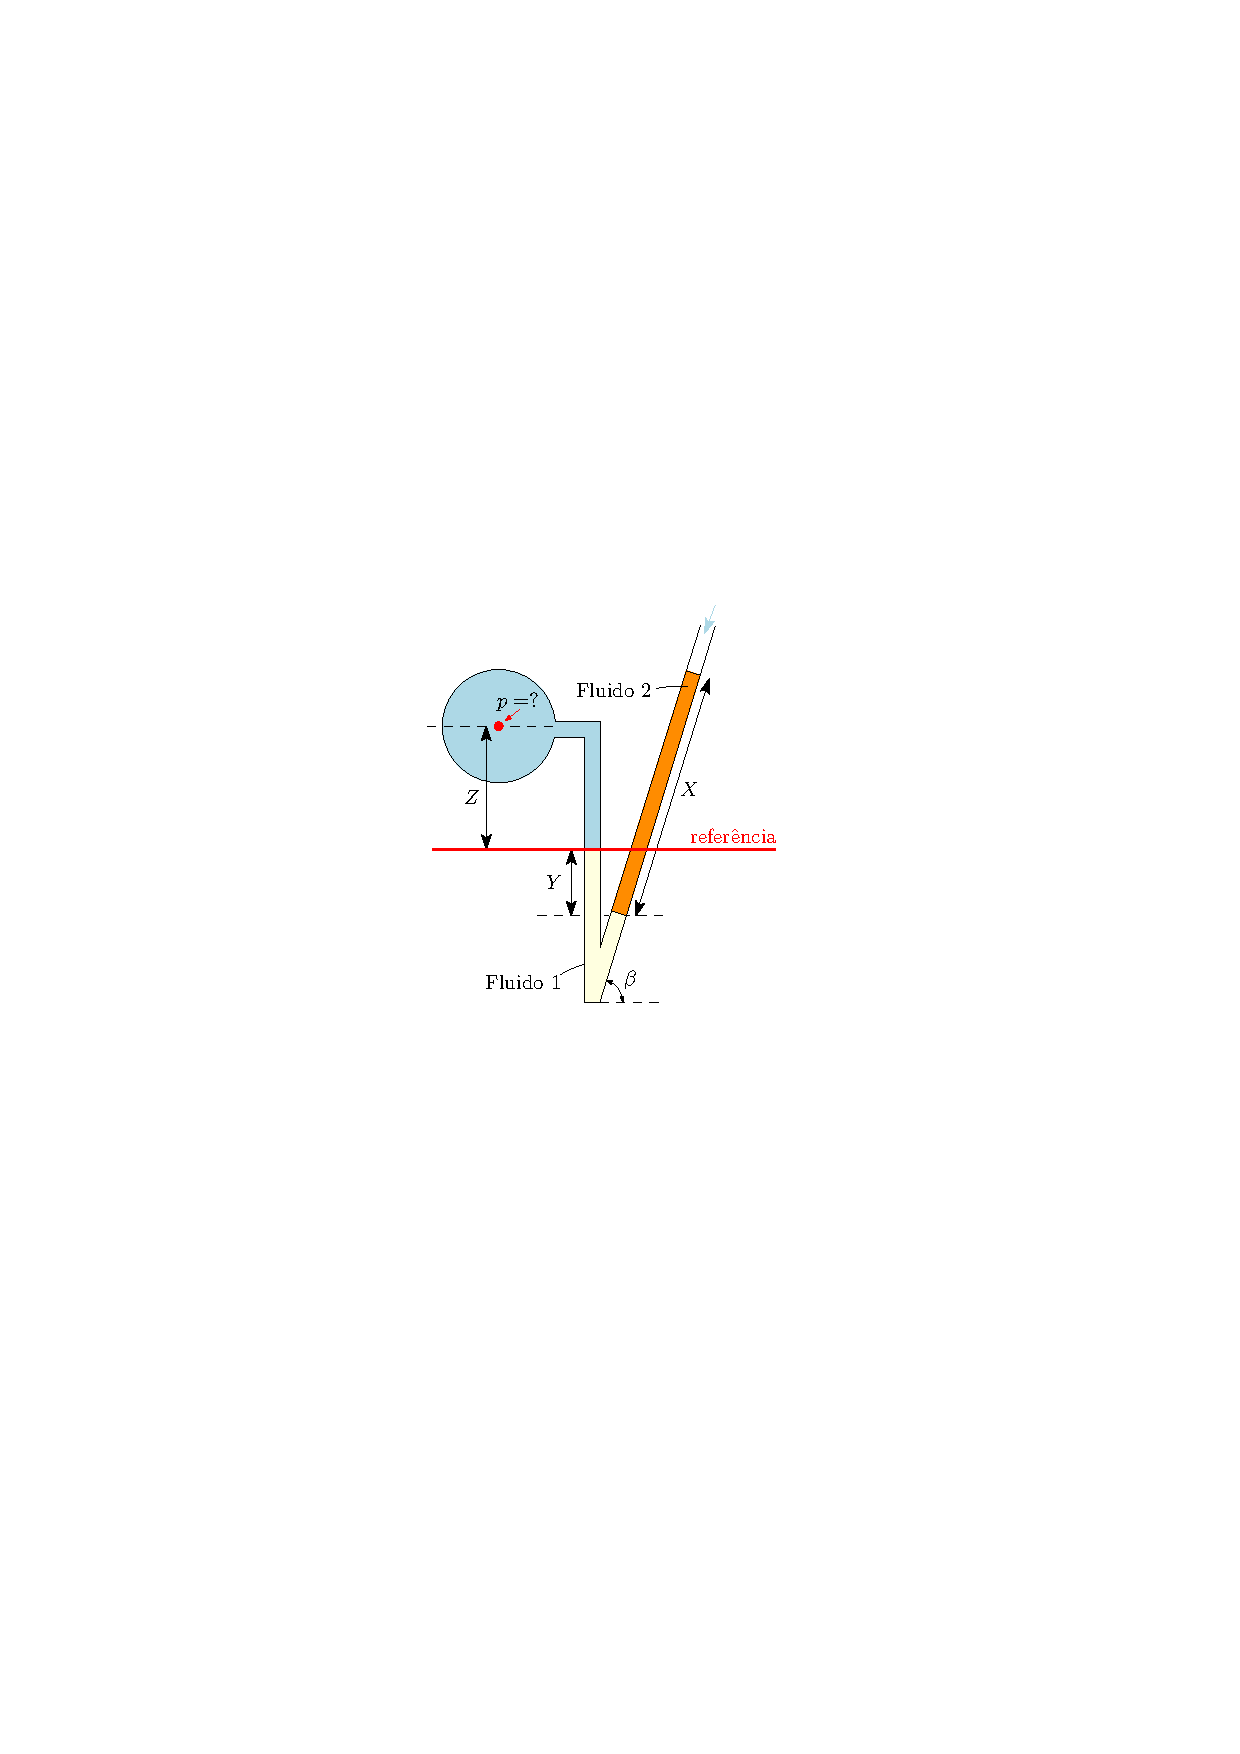
\includegraphics[width=.5\linewidth]{assets/images/referencia}
		\end{center}
		\item[(2)] Após estabelecer a cota de referência deve-se demarcar os pontos que serão analisados quanto a variação de pressão. Nesse caso, foram definidos dois pontos pertencentes à cota (1 e 2) e um ponto na superfície superior do fluido 2 (3) já que a pressão atmosférica na região simplifica os cálculos.
		\begin{center}
			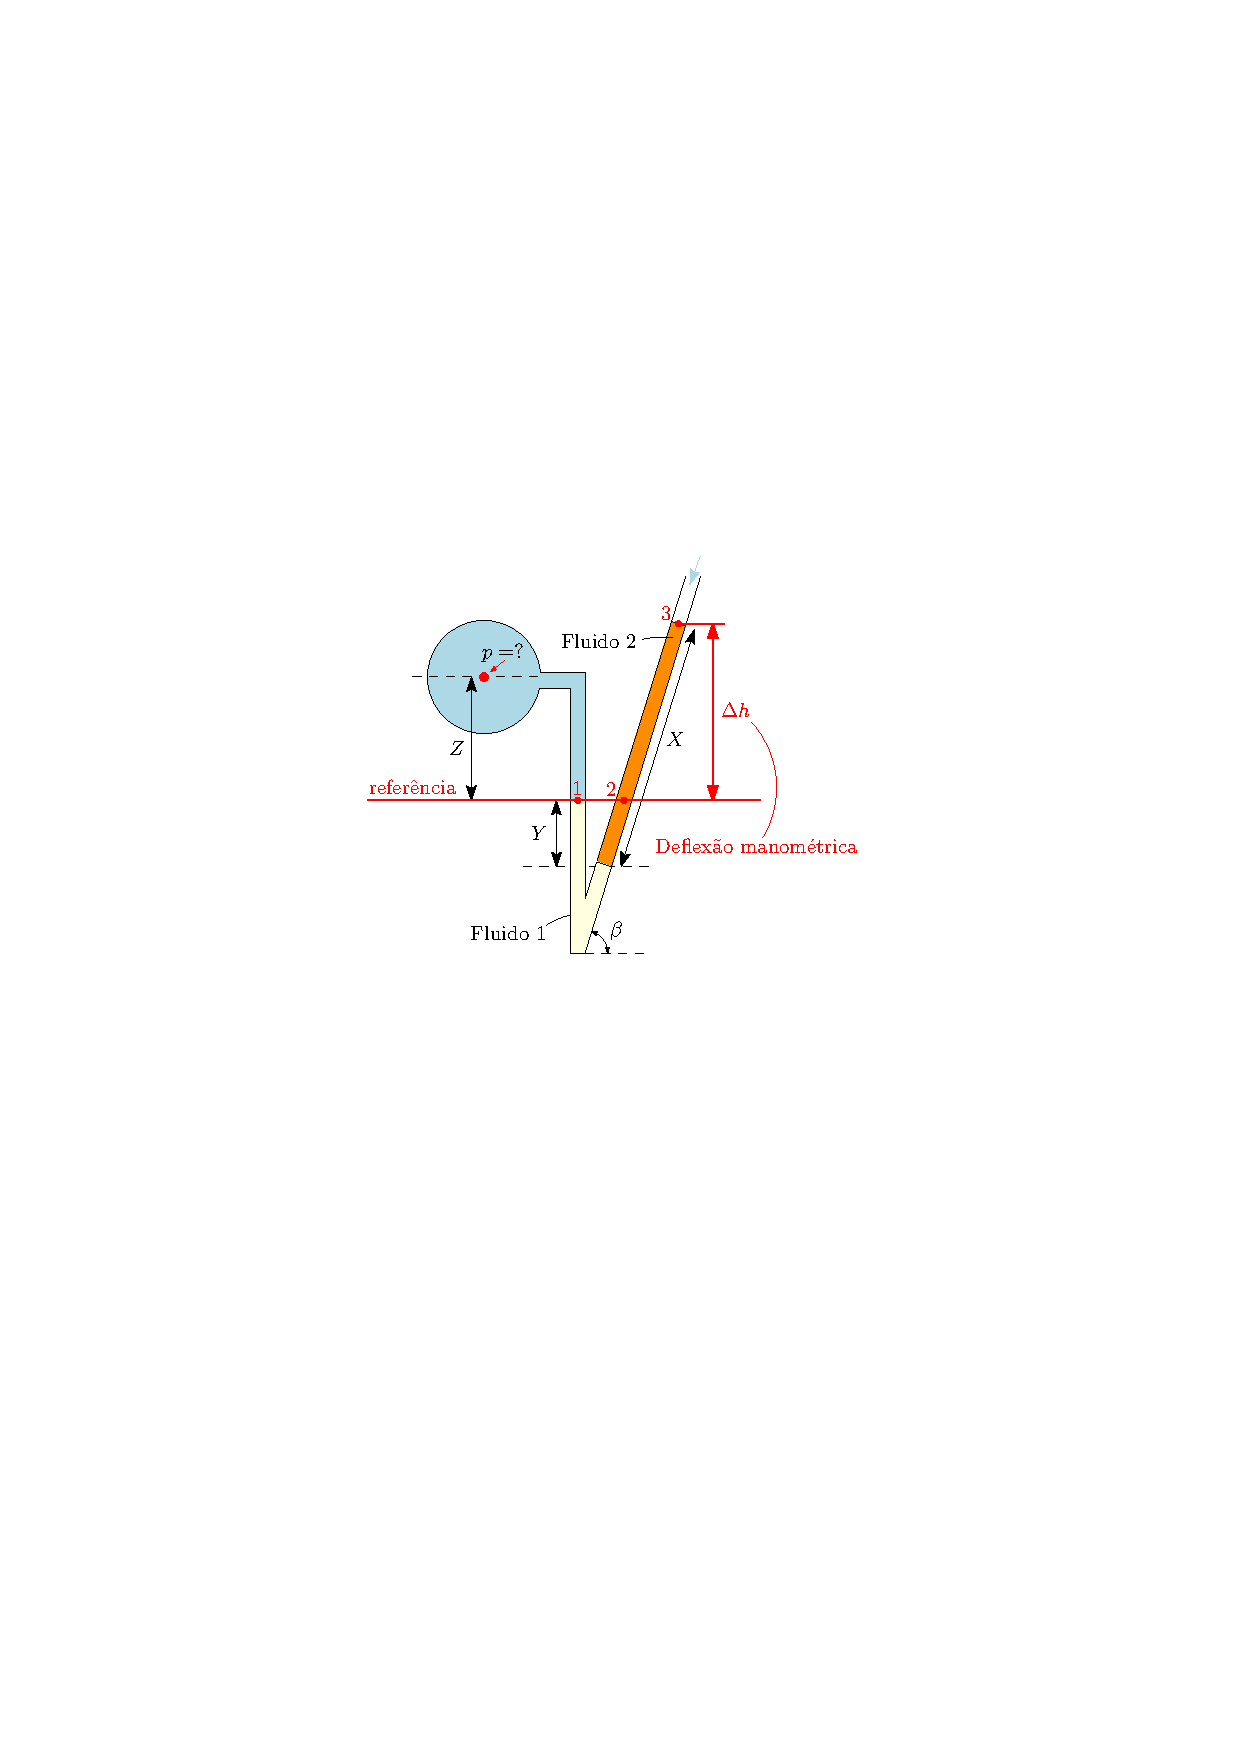
\includegraphics[width=.7\linewidth]{assets/images/pontos}
		\end{center}
		\item[(3)] Agora basta aplicar a lógica assimilada na parte de manômetros diferenciais e formular as equações para cada par de pontos como é visto abaixo
		$$
		\begin{cases}
			p_{1}-p=\gamma_{\ce{H2O}}\cdot Z\\
			p_{2}-p_{3}=\gamma_{2}\cdot\Delta h
		\end{cases}
		$$
		\item[(4)] Aplicando os conceitos vistos em hidrostática, sabemos que pontos na mesma cota apresentam a mesma pressão (1 e 2), logo
		\begin{eqnarray}
			p_{1}&=&p_{2}\\
			p+\gamma_{\ce{H2O}}\cdot Z&=&p_{3}+\gamma_{2}\cdot\Delta h
		\end{eqnarray}
		\item[(5)] Como a pressão atuante em 3 é a atmosférica podemos desprezá-la para o sistema analisado, assim ao isolar $p$ obtemos
		\begin{eqnarray}
			p=\gamma_{2}\cdot\Delta h-\gamma_{\ce{H2O}}\cdot Z
		\end{eqnarray}
		\item[(6)] Podemos considerar, por trigonometria, que $\Delta h=X\cdot\sin (\beta)-Y$ e que $\gamma=\rho\cdot g$, então
		\begin{eqnarray}
			p&=&\rho_{2}\cdot g\cdot (X\cdot\sin(\beta)-Y)-\rho_{\ce{H2O}}\cdot g\cdot Z\\
			&=&g\cdot\big(\rho_{2}\cdot (X\cdot\sin(\beta)-Y)-\rho_{\ce{H2O}}\cdot Z\big)
		\end{eqnarray}
		\item[(7)] Por fim, é necessário considerar as unidades no SI e converter as massas específicas dadas em gramas por centímetro cúbico ($\SI{}{\gram/\centi\meter^{3}}$) para quilogramas por metro cúbico ($\SI{}{\kilogram/\meter^{3}}$)
		\begin{eqnarray}
			\SI{}{\dfrac{\gram}{\centi\meter^{3}}}&=&\dfrac{10^{-3}}{(10^{-2})^{3}}\SI{}{\dfrac{\kilogram}{\meter^{3}}}\\
			&=&\dfrac{10^{-3}}{10^{-6}}\SI{}{\dfrac{\kilogram}{\meter^{3}}}\\
			&=&\SI{1000}{\dfrac{\kilogram}{\meter^{3}}}
		\end{eqnarray}
		\item[(8)] Ao multiplicar os valores de massa específica em gramas por centímetro cúbico por 1000 e substituir o restante dos valores de comprimento (em metros) na equação obtida para $p$, obtemos que $p$ será
		\begin{eqnarray}
			p&=&9.81\cdot\big(8300\cdot(18.4\cdot 10^{-2}\cdot\sin\SI{67.4}{\SIUnitSymbolDegree}-8.3\cdot 10^{-2})-\\
			&-&1000\cdot 21.9\cdot 10^{-2}\big)\\
			&=&\SI{4924.9}{\pascal}\approx\SI{4.9}{\kilo\pascal}
		\end{eqnarray}
	\end{enumerate}
	\section{Segunda questão}
	
	A figura abaixo ilustra um reservatório de água, cujo nível $h$ pode ser determinado utilizando um manômetro. Calcule o valor de $h$ em centímetros (\SI{}{\centi\meter}) com uma casa decimal.\\\vspace{.5cm}
	
	\textbf{Dados:}
	\begin{itemize}
		\item Reservatório contém água
		\item Manômetro contém líquido\\ manométrico: Mercúrio
		\item Peso específico da água:\\ $\gamma_{\ce{H2O}}=\SI{1000}{kgf/\meter^{3}}$
		\item Peso específico do mercúrio:\\ $\gamma_{\ce{Hg}}=\SI{13600}{kgf/\meter^{3}}$
		\item $x=\SI{29.2}{\centi\meter}$
		\item $y=\SI{10.9}{\centi\meter}$
	\end{itemize}
	\vspace{-7.5cm}
	\begin{flushright}
		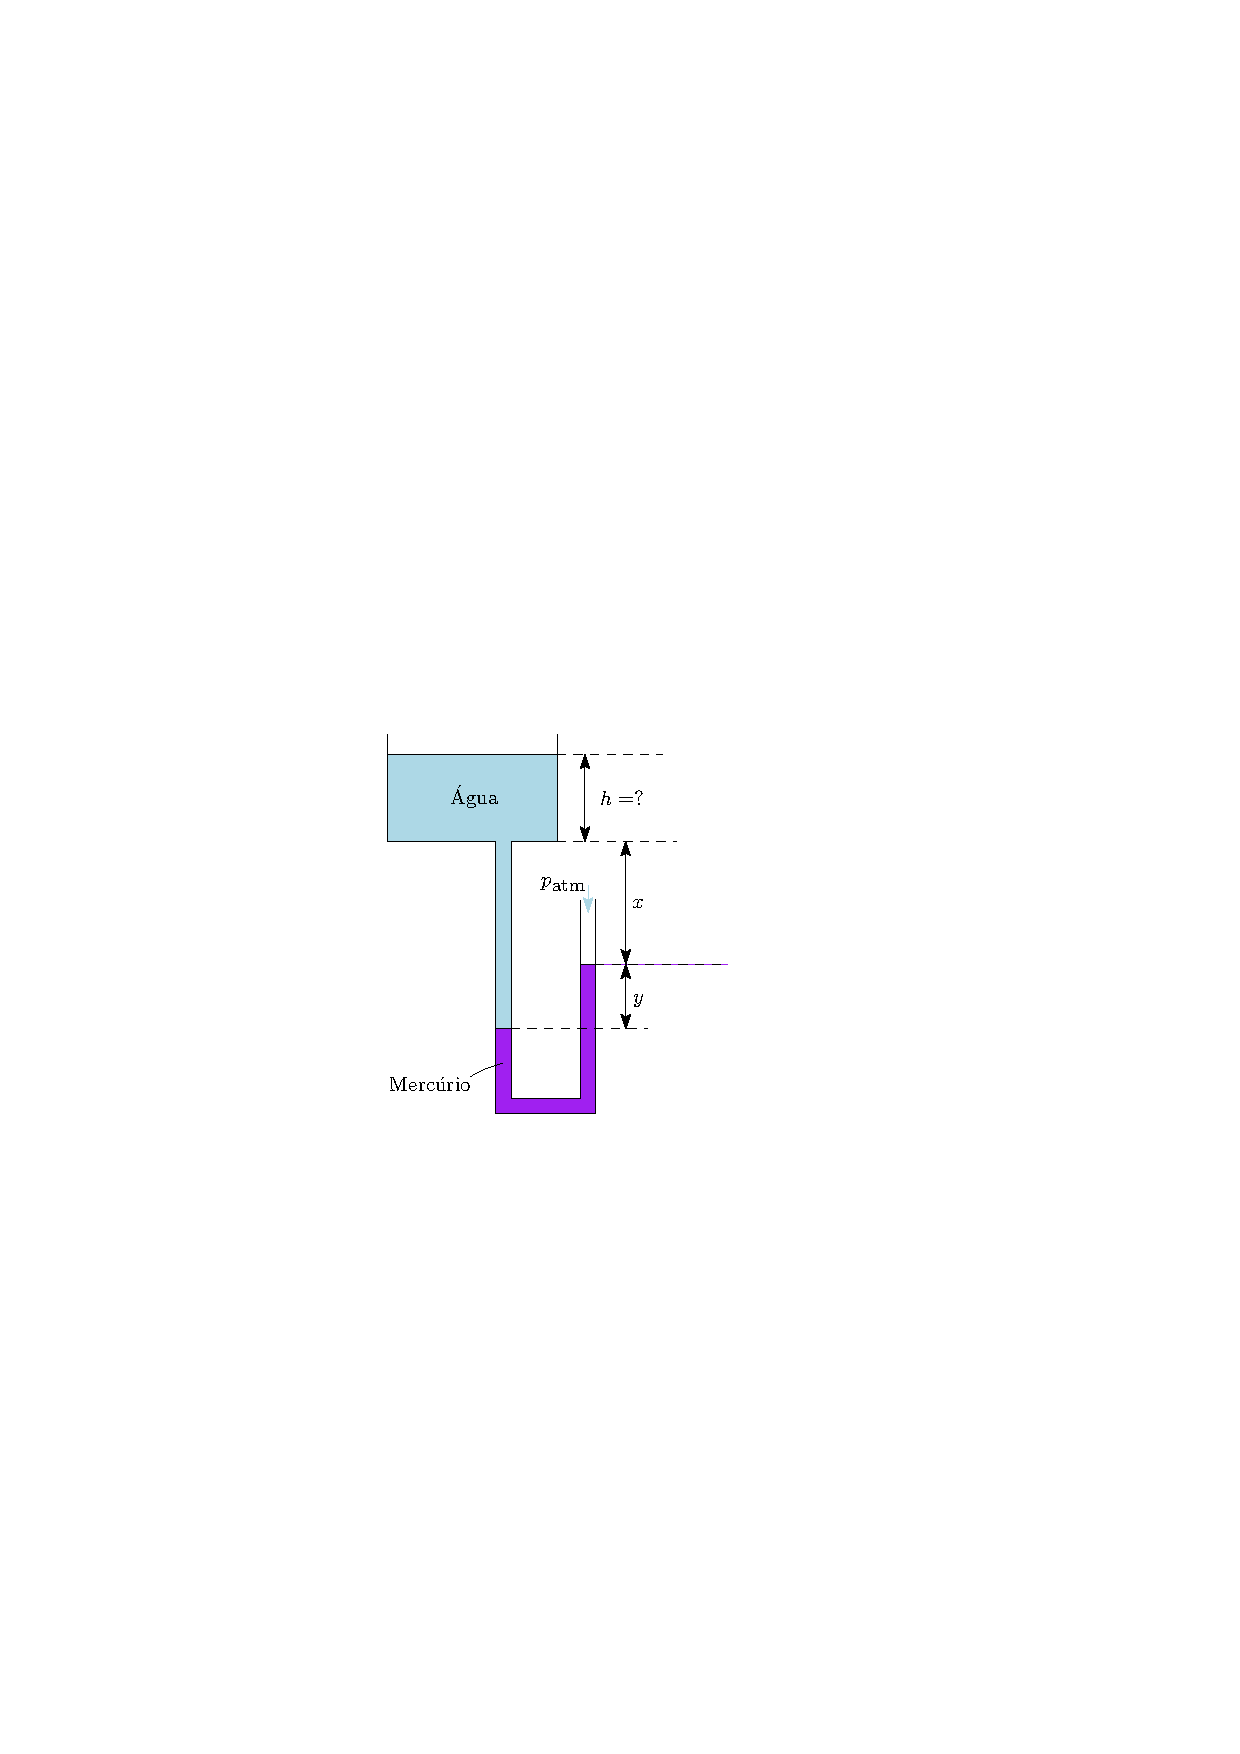
\includegraphics[width=.45\linewidth]{assets/images/ex2}
	\end{flushright}
	\begin{enumerate}
		\item[(1)] De maneira análoga a que foi usada na questão anterior, foi feito o estabelecimento de uma cota de referência e a marcação dos pontos para formular as equações
		\begin{center}
			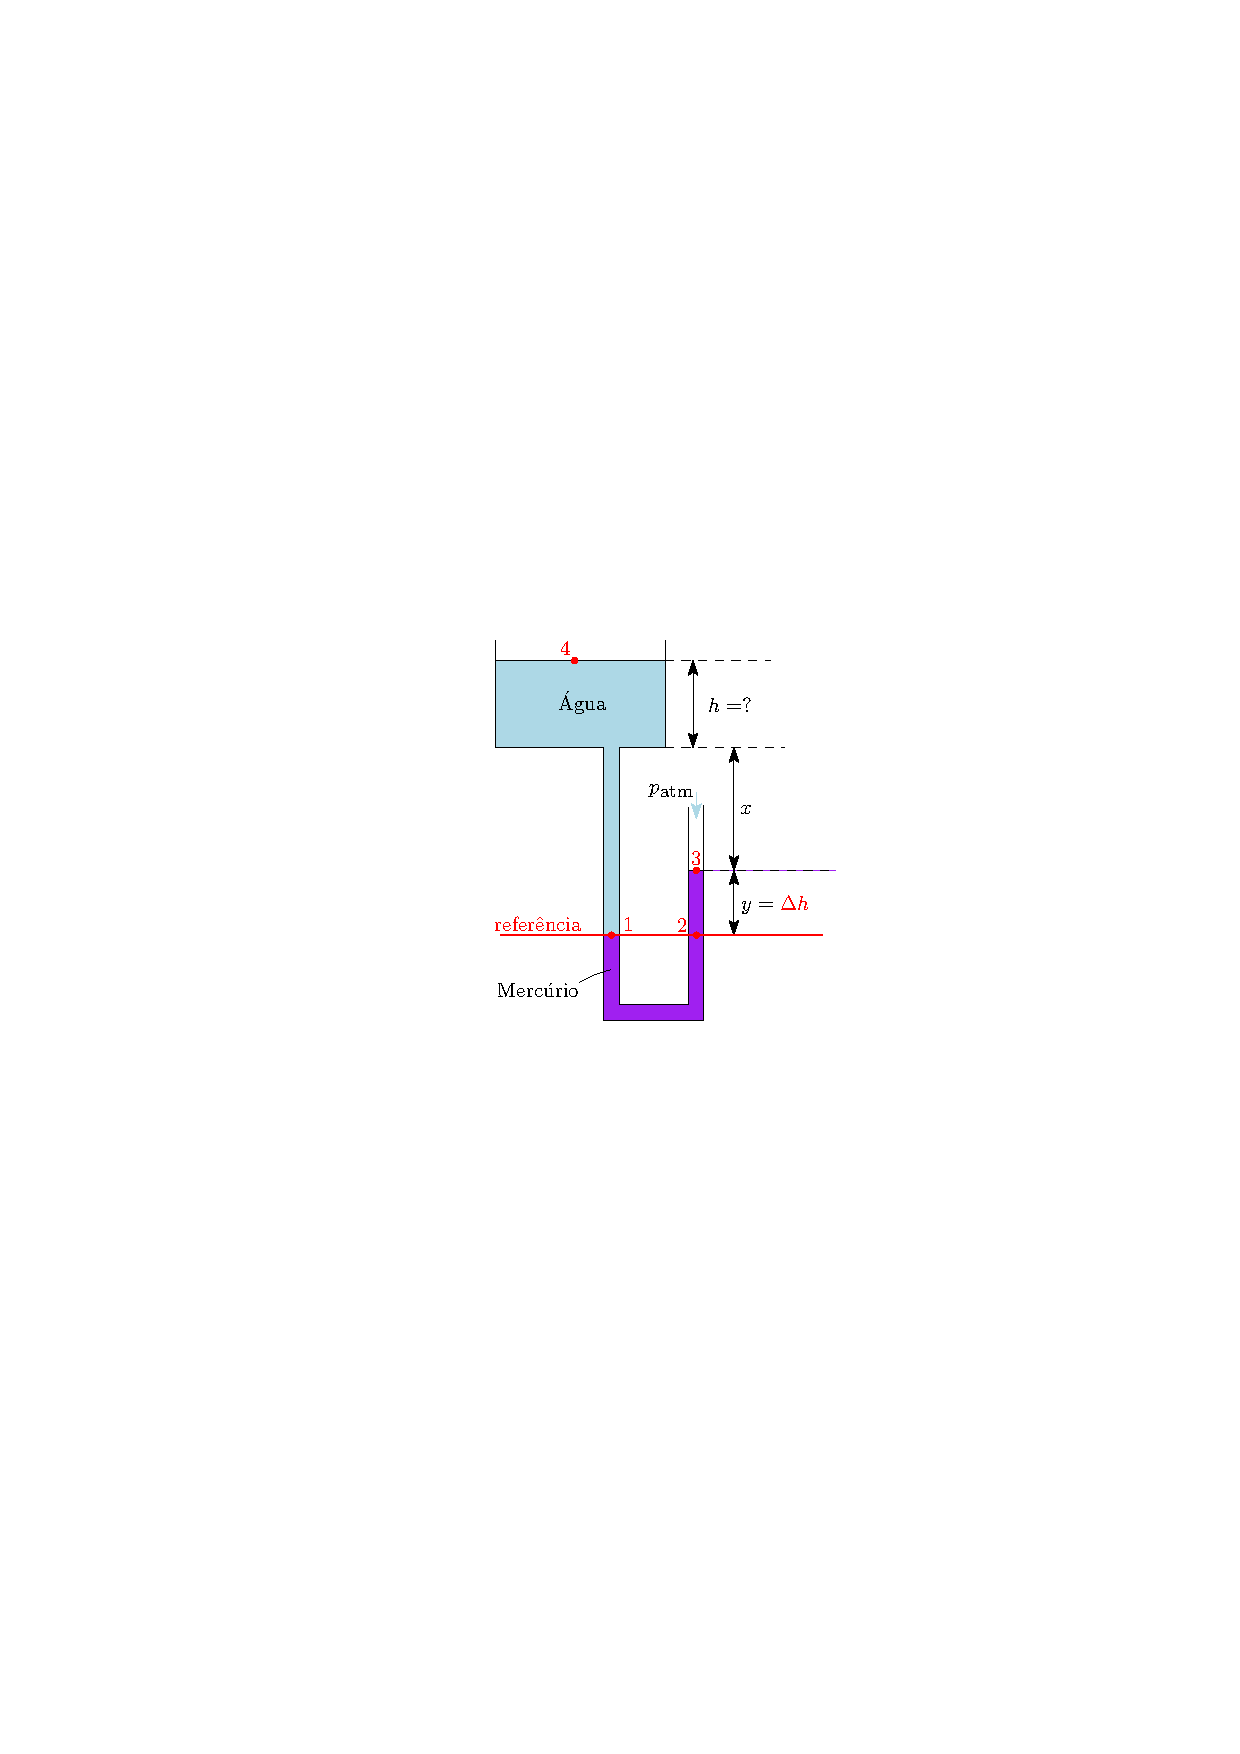
\includegraphics[width=.5\linewidth]{assets/images/referencia_2}
		\end{center}
		\item[(2)] As equações obtidas são
		$$
		\begin{cases}
			p_{1}-p_{4}=\gamma_{\ce{H2O}}\cdot (x+y+h)\\
			p_{2}-p_{3}=\gamma_{\ce{Hg}}\cdot y
		\end{cases}
		$$
		Assim
		\begin{eqnarray}
			p_{1}&=&p_{2}\\
			\gamma_{\ce{H2O}}\cdot (x+y+h)&=&\gamma_{\ce{Hg}}\cdot y\\
			h&=&\dfrac{(\gamma_{\ce{Hg}}-\gamma_{\ce{H2O}})\cdot y-\gamma_{\ce{H2O}}\cdot x}{\gamma_{\ce{H2O}}}
		\end{eqnarray}
	\end{enumerate}
	Considerando que 
	\begin{equation}
		\SI{1}{kgf}=\SI{9.81}{\newton}
	\end{equation}
	temos
	\begin{eqnarray}
		h&=&\dfrac{\cancel{9.81}\cdot (13600-1000)\cdot 10.9\cdot 10^{-2}-\cancel{9.81}\cdot 1000\cdot 29.2\cdot 10^{-2}}{\cancel{9.81}\cdot 1000}\\
		&=&\SI{1.0814}{\meter}\approx\SI{108.1}{\centi\meter}
	\end{eqnarray}
\end{document}